\begin{figure*}
\begin{center}

\begin{minipage}{0.75\textwidth}
\begin{subfigure}[b]{\columnwidth}
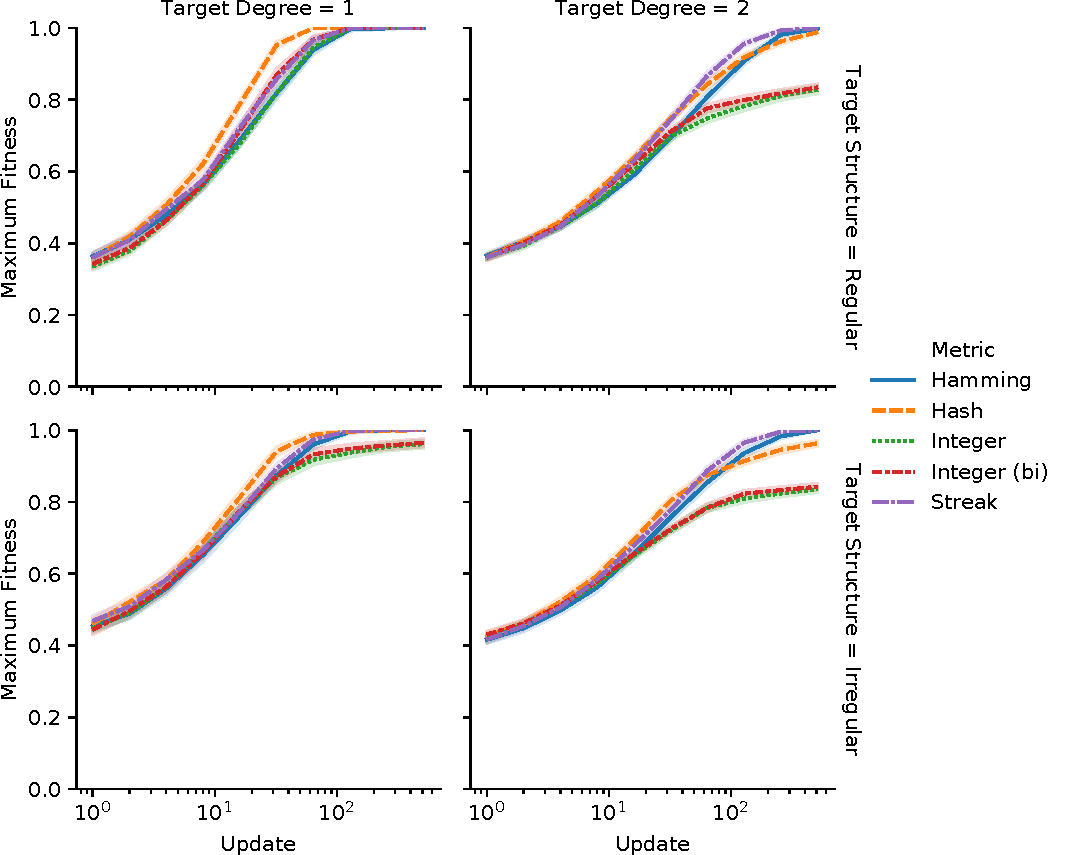
\includegraphics[width=\textwidth]{{{target_evolve/viz=max-fitness-line+_data_hathash_hash=673d309ab90e91d1+_script_fullcat_hash=fe3ddc711c5abfad+ext=}}}
\caption{32-node target graph}
\label{fig:evolve_small_bests}
\end{subfigure}
\begin{minipage}{\textwidth}
~
~
~
~
\end{minipage}
\begin{subfigure}[b]{\columnwidth}
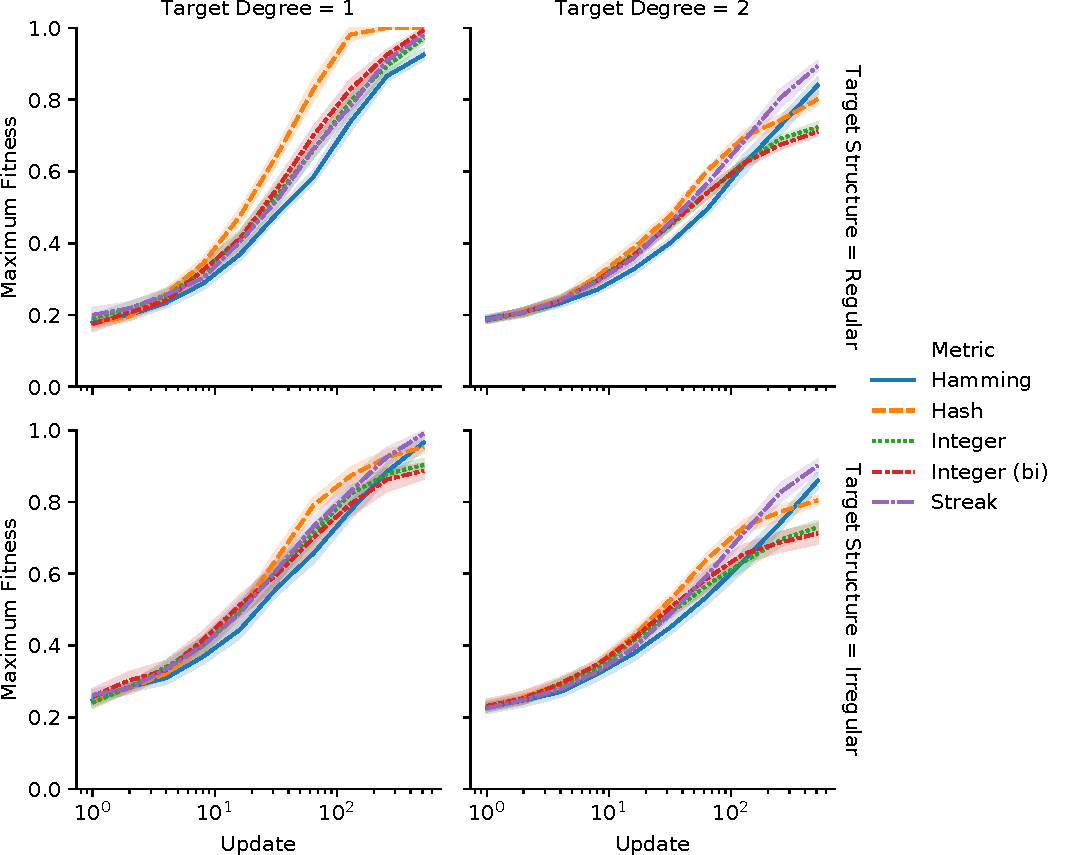
\includegraphics[width=\textwidth]{{{target_evolve_big/viz=max-fitness-line+_data_hathash_hash=4db1200f9d71a980+_script_fullcat_hash=fe3ddc711c5abfad+ext=}}}
\caption{64-node target graph}
\label{fig:evolve_big_bests}
\end{subfigure}
\end{minipage}%
\begin{minipage}{0.25\textwidth}
\caption{
Maximum fitness by update over replicate runs for each metric's best-performing mutation rate.
Note log-scale x-axes.
Shaded area represents 95\% confidence intervals.
}
\label{fig:evolve_bests}
\end{minipage}
\end{center}
\end{figure*}
